\documentclass[10pt,a4paper]{article}
\usepackage[margin=1in]{geometry}
\usepackage{todonotes}
%\setuptodonotes{inline,color=blue!25,tickmarkheight=25mm,size=\small}
\setuptodonotes{
  inline,
  color=blue!25,           % Background color
  backgroundcolor=blue!25, % Same as color (alternative name)
  size=\small,            % \tiny, \scriptsize, \footnotesize, \small, \normalsize, etc.
  tickmarkheight=10mm,     % Height of margin marker
}

\usepackage[T1]{fontenc}
\usepackage{amssymb}
\usepackage{amsthm}
\usepackage{physics}
\usepackage[dvipsnames]{xcolor} %colors
\usepackage{float} % <- importante
\usepackage[draft,inline,nomargin]{fixme} \fxsetup{theme=color} % Comments
\definecolor{jacolor}{RGB}{200,40,0}
\FXRegisterAuthor{ja}{aja}{\color{jacolor}JA}

\usepackage{hyperref}
\hypersetup{
colorlinks=true,
linkcolor=blue,
filecolor=blue,      
citecolor=blue,
urlcolor=blue,
pdftitle={},
pdfauthor=author={},
}

\usepackage[
backend=bibtex,
style=phys,
maxbibnames=5,
biblabel=brackets,
hyperref=true,
arxiv=abs,
eprint=true,
url=false,
doi=false
]{biblatex}
\AtEveryBibitem{\clearfield{note}}
\AtEveryBibitem{\clearfield{pubstate}}  % Remove pubstate from all entries
\addbibresource{symmetries_and_chaos.bib} 
\graphicspath{{img/}}
\newcommand{\eref}[1]{eq.~(\ref{#1})} 
\newcommand{\sref}[1]{sec.~\ref{#1}}
%\newcommand{\tref}[1]{table~\ref{#1}}
\newcommand{\Eref}[1]{Eq.~(\ref{#1})} 
\newcommand{\Sref}[1]{Sec.~\ref{#1}}
\newcommand{\Appref}[1]{Appendix~\ref{#1}}
\newcommand{\Fref}[1]{Fig.~\ref{#1}}  
\newcommand{\Tref}[1]{Table~\ref{#1}}

\title{Survival probability}

\begin{document}
\maketitle
\tableofcontents

\listoftodos

\pagebreak

\section{Question}
Why is the correlation hole not affected by the precense of a high degree
of symmetries in Ref.~\cite{delacruz_2020_quantum}?

\section{Mostly ideas}
\subsection{Survival probability in a system with the simplest symmetric structure}
The survival probability is defined as 
\begin{equation}
S_p(t)
= 
\abs{\braket{\psi_0}{\psi(t)}}^2,
\end{equation}
Consider that $H \ket{\phi_n} = E_n \ket{\phi_n}$, then the survival probability
$S_p$ yields
\begin{equation}
S_p(t) 
= 
\abs{
\sum_{k}
\abs{\braket{\psi_0}{\phi_k}}^2
e^{-i E_k t}
}^2.
\end{equation}
Let us consider a symmetry of $H$ under an arbitrary operator $\Pi$ such 
that $H = H_1 \oplus H_2$---for instance, you may consider $\Pi$ to be the 
reflection operator. Then, we can relabel the energies $E_n$ such that 
$\{E_n\}_{n=1}^p$ and $\{E_n\}_{n=p+1}^N$ are the spectra of $H_1$ and 
$H_2$, respectively. $N$ denotes the dimension of $H$, $p$ the dimension of 
$H_1$ and $N-p$ is the dimension of $H_2$. After this relabeling, $S_p(t)$
takes the form:
\begin{align}
S_p(t) 
&=
\abs{
\sum_{k = 1}^p
\abs{\braket{\psi_0}{\phi_k}}^2
e^{-i E_k t}
+
\sum_{l = p+1}^N
\abs{\braket{\psi_0}{\phi_l}}^2
e^{-i E_l t}
}^2 \\
%
&= 
\abs{
\sum_{k = 1}^p
\abs{\braket{\psi_0}{\phi_k}}^2
e^{-i E_k t}
}^2 
+
\abs{
\sum_{l = p+1}^N
\abs{\braket{\psi_0}{\phi_l}}^2
e^{-i E_l t}
}^2 \\
&\quad +
2\Re{
\sum_{k=1}^{p+1}\sum_{l = p+1}^N
\abs{\braket{\psi_0}{\phi_k}}^2
\abs{\braket{\psi_0}{\phi_l}}^2
e^{-i(E_k - E_l) t}
}.
\end{align}
The first two terms are recognized as the survival probability in the two
symmetric subspaces. The third term God knows what the hell it is, but it 
is the term explaining why the correlation whole survives (or not).

\subsection{Survival probability as function of level spacings}
Let us rewrite the survival probability as follows:
\begin{align}
S_p(t) 
&= 
\abs{
\sum_{k}
\abs{\braket{\psi_0}{\phi_k}}^2
e^{-i E_k t}
}^2 
\\
%
&= 
\sum_{k,l}
\abs{\braket{\psi_0}{\phi_k}}^2
\abs{\braket{\psi_0}{\phi_l}}^2
e^{-i (E_k - E_l) t} \\
%
&= 
\sum_{k=1}^N
\abs{\braket{\psi_0}{\phi_k}}^2
\abs{\braket{\psi_0}{\phi_k}}^2
+ 2\Re\Bigg[
\sum_{k=1}^{N-1}
\abs{\braket{\psi_0}{\phi_k}}^2
\abs{\braket{\psi_0}{\phi_{k+1}}}^2
e^{-i (E_k - E_{k+1}) t} 
\nonumber \\
%
&\quad\, + 
\sum_{k=1}^{N-2}
\abs{\braket{\psi_0}{\phi_k}}^2
\abs{\braket{\psi_0}{\phi_{k+2}}}^2
e^{-i (E_k - E_{k+2}) t} 
+ \ldots
\nonumber \\
%
&\quad\, + 
\abs{\braket{\psi_0}{\phi_N}}^4
e^{-i (E_1 - E_N) t} \Bigg]. 
\label{eq:Sp:spacings}
\end{align}
In this form, it is explicit that the survival probability can be written
as a sum of the contributions given by higher order spacings. From 
Ref.~\cite{tekur_2020_symmetry} we learned not only that RMT's predictions
can be verified even a non-desymmetrized system, but also that higher 
order spacing ratios exhibit correlations that match RMT's predictions.
Very recently, a work on the distribution of higher order spacings
for the circular gaussian ensembles appeared on the 
arXiv~\cite{rout_2025_higherorder} 
\janote{I think these results we can use them to study
the behavior of each term in Eq.~\eqref{eq:Sp:spacings}. My guess is that 
the most relevant contributions to $S_p(t)$ come from the higher order 
spacing correlations}.

Let us consider two identical spectra $\{E^{(1)}_1, E^{(1)}_2, E^{(1)}_3\}$
and $\{E^{(2)}_1, E^{(2)}_2, E^{(2)}_3\}$ (that is, $E^{(1)}_i = E^{(2)}_i$).
The whole ordered spectrum will be 
$\{E^{(1)}_1, E^{(2)}_1, E^{(1)}_2, E^{(2)}_2, E^{(1)}_3, E^{(2)}_3\}$.
Then, compute the spacings:
\begin{align}
s^{(1)}_1 &= E^{(2)}_1 - E^{(1)}_1 = 0\\
s^{(2)}_1 &= E^{(1)}_2 - E^{(1)}_1 \\
s^{(3)}_1 &= E^{(2)}_2 - E^{(1)}_1 \\
s^{(4)}_1 &= E^{(1)}_3 - E^{(1)}_1 \\
s^{(5)}_1 &= E^{(2)}_3 - E^{(1)}_1 
\end{align}
The spacings of first order $s_n^{(1)}$ follow a Poissonian distribution, 
possibly a zero-inflated Poisson distribution as half the spacings will 
become zero. The second-order spacings become the first-order spacings 
of both subspaces \janote{I think the PDF here will be the convolution of 
two Wigner surmises}. The third-order spacings become a mix between first-
and second-order spacings \janote{maybe the convolution of three Wigner surmises?}. The fourth-order spacings will become second-order spacings from
both subspaces\janote{once again, the convolution of four Wigner surmises?}.
The fifth-order spacings become a mix between second- and third-order 
spacings\janote{you know the drill by now, the convolution of five Wigner 
surmises?}

\janote{I guess the convolution of many Wigner surmises should converge to
something...? Hence, after some order the PDF should be almost the same.
Something to ask Deepseek or chatGPT}

\janote{If all of this is, at the very least, a good approximation, we still 
have to take into account the coefficients $\abs{\braket{\psi_0}{\phi_i}}^2
\abs{\braket{\psi_0}{\phi_{i+k}}}^2$.
Therefore, we may consider the case where all coefficients are equal, case
in which I'm almost sure the $S_p(t)$ becomes the spectral form factor. If it 
is indeed the case we should expect a dip-ramp-plateau behavior, the ramp being 
the hallmark of long-range correlations of a spectrum's chaotic system.
}

\subsection{Spectral form factor (SFF)}
The SFF can be decomposed into the following sums:
\begin{align}
\label{eq:sff}
K(t) &= \frac{1}{N^2} \overline{\sum_{k,l} e^{-i (E_k - E_l) t}} \\
&= 
1
+ \frac{2}{N^2}\Re\Bigg[
\overline{
\sum_{k=1}^{N-1}
e^{-i (E_{k+1} E_k) t} 
} +
\overline{
\sum_{k=1}^{N-2}
e^{-i (E_{k+2} - E_k) t} 
}
+ \ldots +
\overline{
e^{-i (E_N - E_1) t} 
}
\Bigg].
\label{eq:sff:spacings}
\end{align}
\todo{SN: As a sanity check, check numerically in the BH model that Eqs. \eqref{eq:sff} and \eqref{eq:sff:spacings} give the same SFF curve, computing separately term by term of \Eref{eq:sff:spacings}, and then adding them up}

We try to move forward with the following approximation. We assume the spacings
$s^{(1)}_k = E_{k+1} - E_k$ are independent and identically distributed 
(i.i.d), thus:
\begin{equation}\label{eq:sff:spacings1}
\overline{
\sum_{k=1}^{N-1}
e^{-i (E_{k+1} E_k) t} 
}
\approx
(N-1) \, \overline{e^{-i s^{(1)} t}} 
= 
\int_0^\infty
e^{- i s t} P(s)
\dd{s},
%= 
%\int_0^\infty
%e^{- i s t} \cdot 
%\frac{\pi s}{2} e^{-\pi s^2 / 4}
%\dd{s}
\end{equation}
where $P(s)$ is either a Poisson or a Wigner-Dyson distribution, 
depending on the case, 
\begin{align}
\label{eq:sff:spacings1:WDapprox}
\int_0^\infty
e^{- i s t} P_{\mathrm{WD}}(s)
\dd{s}
&=
(N-1)\left[1 - t e^{-t^{2}/\pi}\left(\mathrm{erfi}\left(\frac{t}{\sqrt{\pi}}\right) + i\right)\right]
\\
%
\label{eq:sff:spacings1:Papprox}
\int_0^\infty
e^{- i s t} P_{P}(s)
\dd{s}
&= 
\frac{N-1}{1+it}.
\end{align}
\todo{SN: Check numerically if the left side of \Eref{eq:sff:spacings1} is well described by either \Eref{eq:sff:spacings1:WDapprox} when a single symmetric subspace is considered, and by \Eref{eq:sff:spacings1:Papprox} when the whole spectrum is considered (we have the intuition that the whole spectrum should exhibit Poisson statistics at first order spacings or ratios)}
\janote{In Ref.~\cite{engel_1998_higherorder} they study the distribution
of higher order level spacings.}

A checking was performed for the proposition made in \Eref{eq:sff:spacings1:WDapprox}:
\begin{figure}[H]
    \centering
    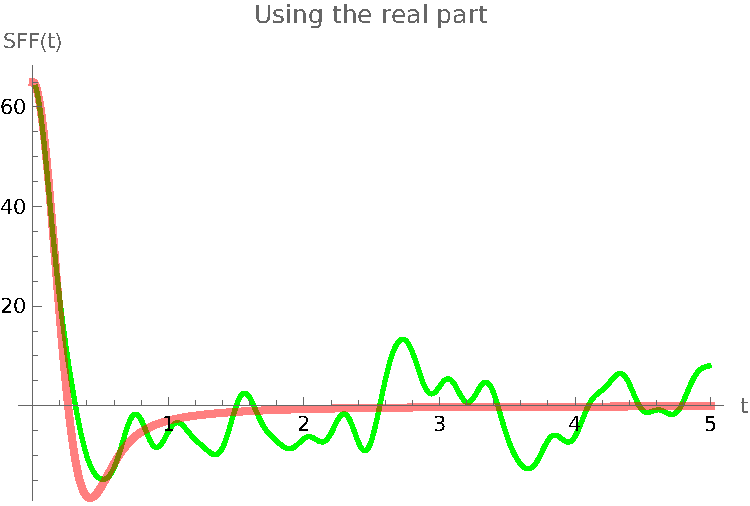
\includegraphics[width=0.5\textwidth]{ApproxWDRe.pdf}
    \caption{Comparing if the left side of \Eref{eq:sff:spacings1} is well described by \Eref{eq:sff:spacings1:WDapprox} when considering a single symmetric subspace. }
    \label{fig:ApproxWDRe}
\end{figure}
\subsection{Interesting things about SFF}
There is a direct need in averanging the SFF computed, here a comparison between two methods will be shown, based on the data 
obtained from the BHH model. A time window averanging is performed on the data and a sector averanging aswell (averanging the SFF at each time with each symmetric sector of the hamiltonian).

The conclusion is that in a general context, a time averanging is best by far in comparison to a sector averanging, mainly due to the 
fact that a hamiltonian might only have 2 symmetric sectors. It is remarkable that applying both a sector averanging and a time window averanging proves to be the most precise approach.
\begin{figure}[H]
    \centering
    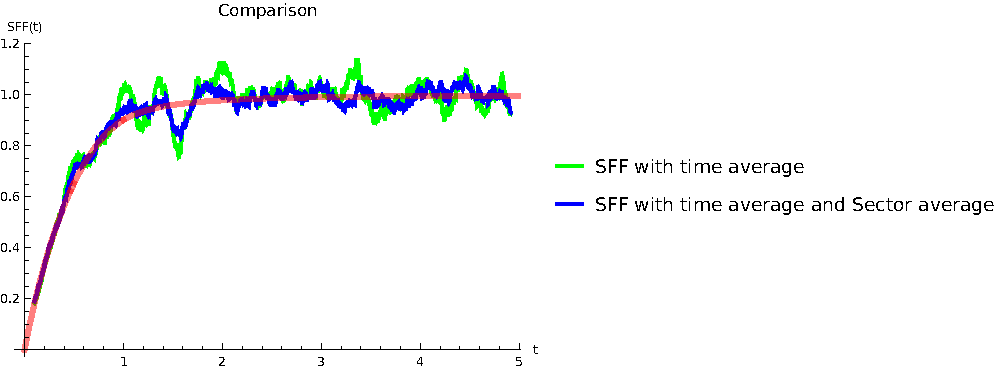
\includegraphics[width=0.9\textwidth]{CompSectAndTime.pdf}
    \caption{Comparison between using just time averanging and time averanging with sector averanging (red line is the GOE prediction).}
    \label{fig:CompSectAndTime}
\end{figure}

Using the GOE, numerical calculations have been performed in order to observe a characteristic behavior that is presented when SFF is considered.
Two approaches where inspected. First, a high order matrix (dimension $\approx 3,000$) that belonged to GOE was generated, with this
a SFF calculation was performed using time averanging.
\begin{figure}[H]
    \centering
    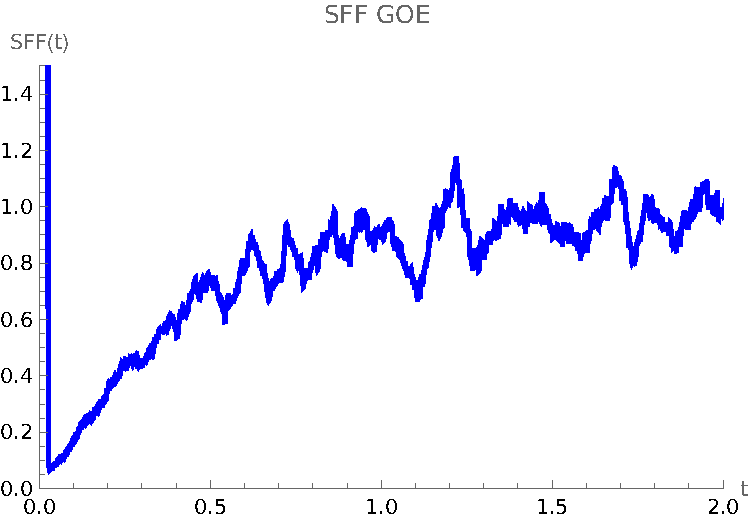
\includegraphics[width=0.7\textwidth]{TAvergGOE.pdf}
    \caption{GOE SFF behavior using time averanging and a GOE matrix of dimension 3000.}
    \label{fig:TAvergGOE}
\end{figure}
Remarkably, using a different approach, where a list of GOE matrices was generated, then a sector averanging with a time averanging was performed,
proving that applying both methodologies proves to be useful (valid only with a decent amount of statistics.)
\begin{figure}[H]
    \centering
    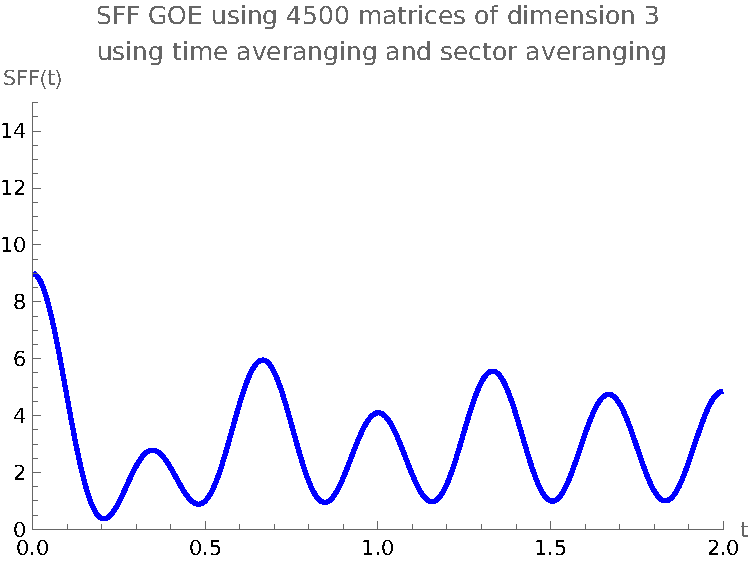
\includegraphics[width=0.7\textwidth]{SFFGOETS3.pdf}
    \caption{GOE SFF behavior using time averanging and sector averanging of a list of 4500 GOE matrices of dimension 3}
    \label{fig:SFFGOETS3}
\end{figure}
\begin{figure}[H]
    \centering
    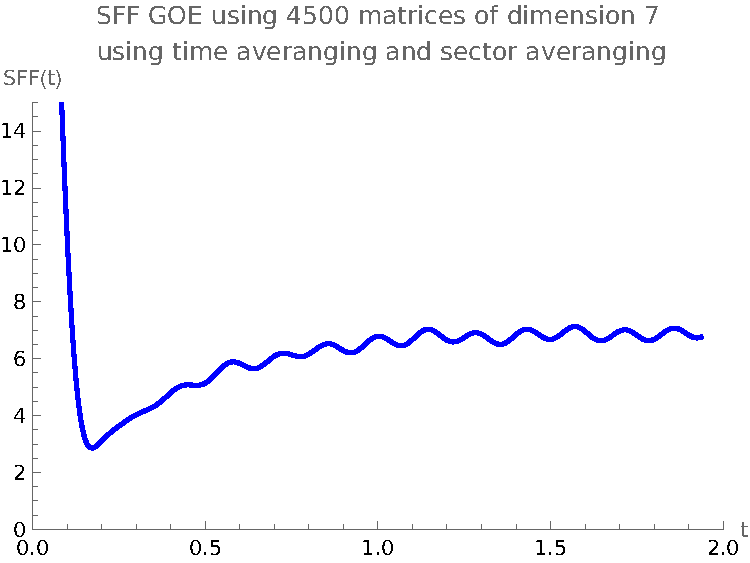
\includegraphics[width=0.7\textwidth]{SFFGOETS7.pdf}
    \caption{GOE SFF behavior using time averanging and sector averanging of a list of 4500 GOE matrices of dimension 7}
    \label{fig:SFFGOETS7}
\end{figure}

\begin{figure}[H]
    \centering
    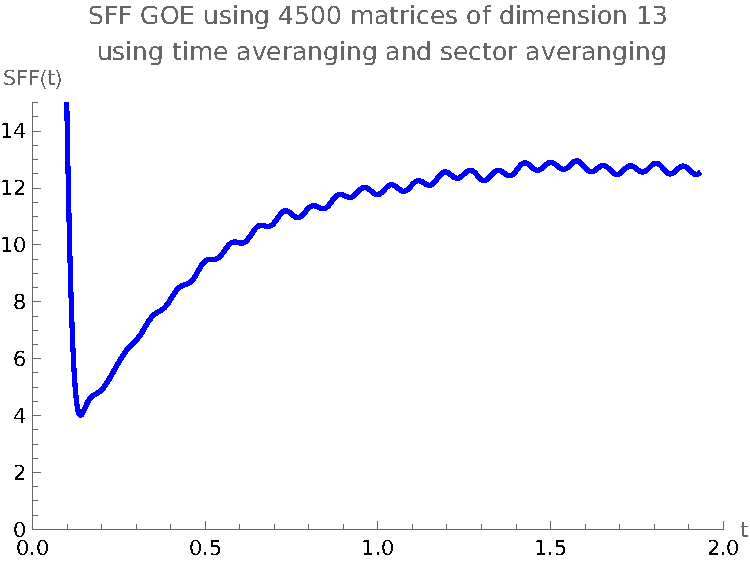
\includegraphics[width=0.7\textwidth]{SFFGOETS13.pdf}
    \caption{GOE SFF behavior using time averanging and sector averanging of a list of 4500 GOE matrices of dimension 13}
    \label{fig:SFFGOETS13}
\end{figure}

\begin{figure}[H]
    \centering
    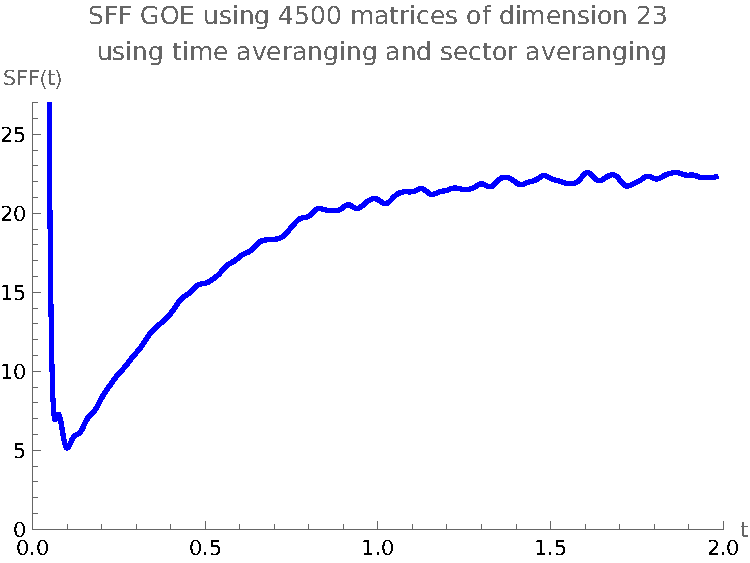
\includegraphics[width=0.7\textwidth]{SFFGOETS.pdf}
    \caption{GOE SFF behavior using time averanging and sector averanging of a list of 4500 GOE matrices of dimension 23}
    \label{fig:SFFGOETS23}
\end{figure}

An observation: It is to be noted that using a high dimension GOE matrix proves to be the most direct way of approaching statistical results,
 an effort must be made on relying in a method that involves a list of low dimensional GOE matrices, due to the fact that 
 a high dimensional matrix might prove a difficutly considering the diagonalization that must be carried eventually.

\section{Mean Spacings Ratio}
Considering the mean spacing ratio of k order proves to be a useful quantity to observe short range correlation, long range correlations 
are difficult to check, and numerical calculation have been performed in order to show that, as k grows, the mean spacing ratio 
value of the GOE becomes indistinguishable from the Poisson prediction, therefore, it is obvious that, above certain k, there is 
no way of distinguishing between GOE or Poisson statistics. The following figure shows the idea, numerical calculation where 
performed for the GOE and for Poisson.

\begin{figure}[H]
    \centering
    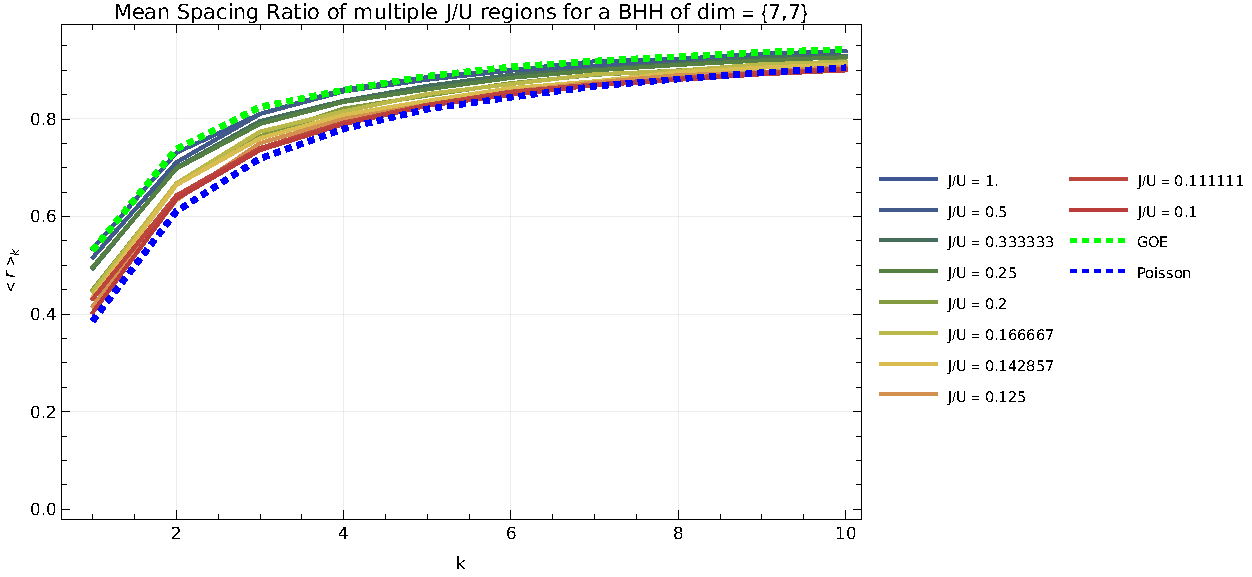
\includegraphics[width=1\textwidth]{KorderCurves.pdf}
    \caption{Mean spacing ratio as k grows of several BHH hamiltonians with different $J/U$ values. }
    \label{fig:KorderCurves}
\end{figure}

\appendix
\section{Average of $\sum_k e^{-i s_k t}$ for Wigner-Surmise Spacings}

We consider the nearest-neighbor spacings $s_k$ distributed according to the \textbf{Wigner surmise}:
\[
p(s) = \frac{\pi s}{2} e^{-\pi s^2 / 4}, \quad s \geq 0.
\]

We wish to compute:
\[
\left\langle \sum_k e^{-i s_k t} \right\rangle.
\]

\subsection*{Assumption}
Assuming the spacings are independent and identically distributed (i.i.d.) with the Wigner surmise distribution:
\[
\left\langle \sum_k e^{-i s_k t} \right\rangle \approx (N-1) \left\langle e^{-i s t} \right\rangle.
\]

\subsection*{Characteristic Function}
The characteristic function is:
\[
\phi(t) = \int_0^\infty e^{-i s t} \, p(s) \, \dd s = \int_0^\infty e^{-i s t} \cdot \frac{\pi s}{2} e^{-\pi s^2 / 4} \dd s.
\]

This integral evaluates to:
\[
\phi(t) = 1 - t e^{-t^2/\pi} \left( \mathrm{erfi}\left( \frac{t}{\sqrt{\pi}} \right) + i \right),
\]
where $\mathrm{erfi}(z) = \frac{2}{\sqrt{\pi}} \int_0^z e^{u^2} \dd u$ is the imaginary error function.

\subsection*{Final Result}
\[
\boxed{\left\langle \sum_k e^{-i s_k t} \right\rangle \approx (N-1)\left[1 - t e^{-t^{2}/\pi}\left(\mathrm{erfi}\left(\frac{t}{\sqrt{\pi}}\right) + i\right)\right]}
\]

\subsection*{Remarks}
\begin{itemize}
    \item This result assumes i.i.d. spacings (a common approximation using the Wigner surmise)
    \item In full RMT (GOE), spacings are not independent, but this captures key features
    \item For $t = 0$: $\phi(0) = 1$ as expected
    \item For small $t$: $\phi(t) \approx 1 - i t - \frac{2}{\pi} t^2 + \cdots$
\end{itemize}

\section{df}
For a quantum system with Poissonian level statistics, the nearest-neighbor spacings $s_k$ are independent and identically distributed with the exponential distribution:
\[
p(s) = e^{-s}, \quad s \geq 0,
\]
where the mean spacing is normalized to unity.

We wish to compute the average:
\[
\left\langle \sum_k e^{-i s_k t} \right\rangle.
\]

Assuming the spacings are independent, this becomes:
\[
\left\langle \sum_k e^{-i s_k t} \right\rangle = (N-1) \left\langle e^{-i s t} \right\rangle,
\]
where the characteristic function is:
\[
\phi(t) = \left\langle e^{-i s t} \right\rangle = \int_0^\infty e^{-i s t} e^{-s} \dd{s} = \int_0^\infty e^{-s(1 + i t)} \dd{s}.
\]

Evaluating this integral gives:
\[
\phi(t) = \frac{1}{1 + i t}.
\]

Therefore, the final result is:
\[
\boxed{\frac{N-1}{1+it}}
\]

\section{A possibly useful integral}
\begin{equation}
\expval{e^{-ist}} =
\frac{1}{2}
e^{-\frac{1}{2} t \left(\sigma ^2 t+2 i\right)} 
\qty[
1 + \erf\qty(\frac{1 - i\sigma^2 t}{\sqrt{2}\sigma})
]
\end{equation}

%!TEX root = main.tex

\section{Poster}
\subsection{Main goal}
The primary objective is to develop an intuitive understanding of the 
correlations associated with higher-order spacings in the Bose-Hubbard (BH) 
model, specifically within the parameter regime characterized by the 
transition from Poisson to Wigner-Dyson statistics suggested by the short-range 
correlation indicators we have previously examined, namely the mean level 
spacing ratio $\ev{r}$ and the Kullback-Leibler (KL) divergence. 
More precisely, I aim to test the hypothesis that long-range correlations emerge gradually, akin to the gradual breakdown of tori in classical chaotic systems as the chaotic parameter is increased.

\subsection{What to do}
Compare the mean spacing ratios of order $k$ of a GOE matrix (sufficiently big)
with that obtained from the BH model. That is, plot $k$ in the horizontal
axis, and $\ev{r^{(k)}}$ in the vertical axis. I would expect that if the 
system is chaotic the curve of GOE and of that of the BH model are the same.
But in the transition between integrable and chaotic, maybe we will observe 
deviations from the GOE? 

%Compare numerically the statistics of higher-order spacings (and ratios if time 
%allows it) of the BH model and matrices sampled from the GOE. 
%
%The spacings of order $k$ $s^{(k)}$ 
%of integrable systems follow a Gamma distribution 
%\begin{equation}
%P_{\mathrm{Poisson}}(s^{(k)})
%= 
%\frac{s^{k-1} e^{-s}}{(k-1)!}
%\end{equation}

\printbibliography
\end{document}